\section{Qualidade do Código Fonte}

\subsection{SonarQube}

\begin{figure}[H]

  \centering

  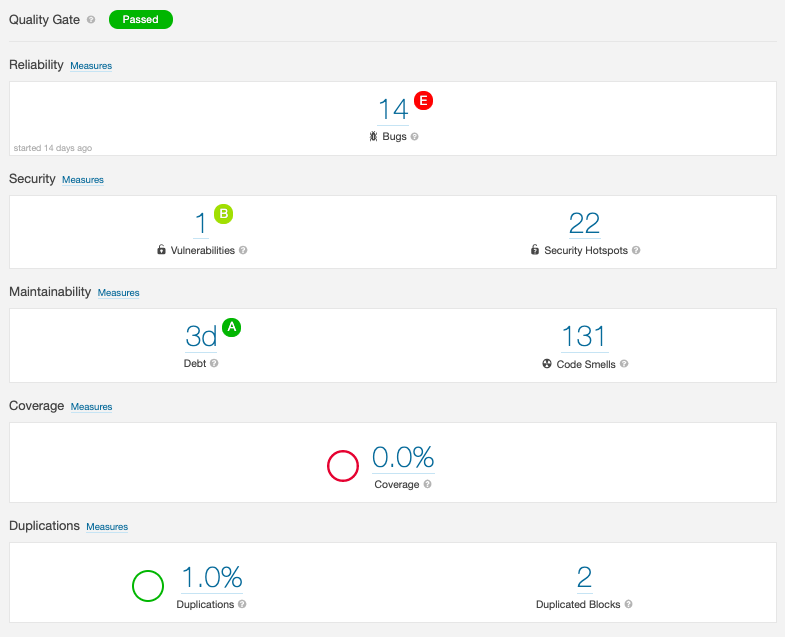
\includegraphics[scale = 0.45]{sonarEvaluation.png}

  \caption {Menu geral de avaliação do SonarQube}

  \label {fig01}

\end{figure}


\par Como se pode ver pela figura~\ref{fig01} este projeto possui alguns bugs, pelo menos 1 vulnerabilidade uma quantidade considerável de \textit{code smells} e 2 blocos duplicados.

\section{Refactoring da Aplicação}

De seguida apresenta-se um relatório detalhado dos tipos de erros e da sua gravidade bem como das respetivas soluções implementadas com recurso ao Eclipse e ao relatório de erros detalhado do \textit{Sonarqube} (incluindo as descrições dos erros e \textit{code smells} encontrados):

\subsection{Bugs}
Versão com e sem \textit{bugs}, com e sem \textit{smells} (por tipos de \textit{smells}) -> descriminar o impacto dos \textit{smells}
\subsubsection{Blocker Bugs:}
\begin{itemize}
\item Não usar blocos \textit{try/catch} ao escrever em ficheiros.\newline
 Ficheiro: UMCarroJa.java\newline


\par Podemos visualizar nas seguintes imagens o código analisado e a solução respetiva.

\begin{figure}[H]

  \centering

  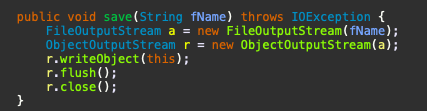
\includegraphics[scale = 0.5]{preWriteTryCatch.png}

  \caption {Código com bug}

  \label {fig02}

\end{figure}

\begin{figure}[H]

  \centering

  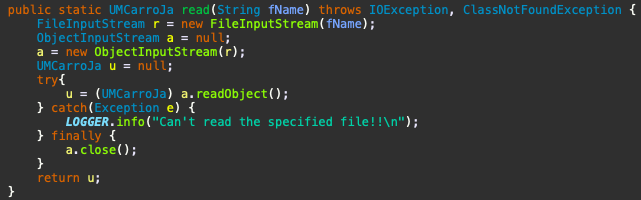
\includegraphics[scale = 0.5]{posreWriteTryCatch.png}

  \caption {Código corrigido}

  \label {fig03}

\end{figure}

\item Não usar blocos \textit{try/catch} ao ler de ficheiros.\newline
 Ficheiro: UMCarroJa.java\newline


\par Podemos visualizar nas seguintes imagens o código analisado e a solução respetiva.


\begin{figure}[H]

  \centering

  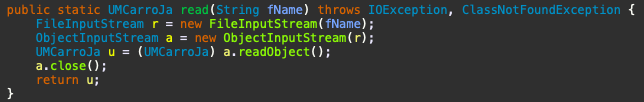
\includegraphics[scale = 0.5]{preReadTryCatch.png}

  \caption {Código com bug}

  \label {fig04}

\end{figure}

\begin{figure}[H]

  \centering

  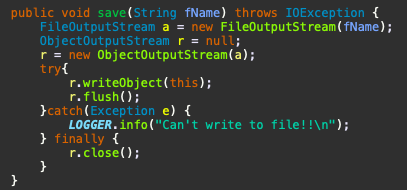
\includegraphics[scale = 0.5]{posreReadTryCatch.png}

  \caption {Código corrigido}

  \label {fig05}

\end{figure}

\end{itemize}
\par Note-se que é usado no fim dos blocos \textit{try/catch} o bloco \textit{finally} para fechar o descritor de escrita/leitura. Isto serve para, caso alguma coisa corra mal na escrita em/leitura de um ficheiro, o descritor ser fechado. 

\subsubsection{Critical Bugs:}
\begin{itemize}
\item Guardar e reutilizar variáveis random.\newline
 Ficheiro: Traffic.java \newline


\par Para resolver o problema basta verificar que o \textit{random} estava a ser gerado sempre que a função \textit{getTraficDelay()} era invocada. Para resolver basta gerar o \textit{random} uma única vez quando a classe for criada e usar o mesmo sempre que a função em causa for invocada.

\begin{figure}[H]

  \centering

  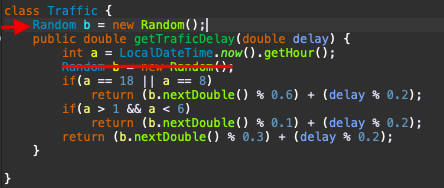
\includegraphics[scale = 0.5]{randomGeneration.png}

  \caption {Recolocação do método de geração de um número \textit{Random}}

  \label {fig06}

\end{figure}
\end{itemize}

\subsubsection{Major Bugs:}
\begin{itemize}
\item Não obrigar a usar o método redefinido usando \textit{override}.\newline
 Ficheiro: Car.java\newline

\par Para resolver este problema da forma mais simples foi preciso renomear o método \textit{equals} para o método \textit{isEqual}, visto que usar um \textit{@Override} sobre este método obrigaria a implementação um método de super tipo e da função \textit{hashCode()}.


\begin{figure}[H]

  \centering

  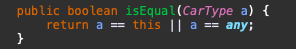
\includegraphics[scale = 0.5]{isEqualFunction.png}

  \caption {Definição da função isEqual}

  \label {fig07}

\end{figure}

\end{itemize}

\subsubsection{Minor Bugs:}
\begin{itemize}
\item Obrigar o override do equals e não o do método \textit{hashCode()}.\newline
 Ficheiros: Car.java, Cars.java, Cliente.java, Owner.java, Parser.java, Rental.java, Rentals.java, User.java, Users.java.\newline


\par Para corrigir este problema, basta definir um \textit{hashCode()} que chame o método \textit{super.hashCode()} como se pode ver na figura seguinte.

\begin{figure}[H]

  \centering

  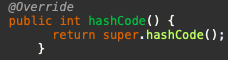
\includegraphics[scale = 0.6]{hashCode.png}

  \caption {Solução do problema de @Override do método hashCode}

  \label {fig08}

\end{figure}

\end{itemize}


\subsection{Vulnerabilitys}
\begin{itemize}
\item Utilizar printStackTrace() pode revelar informação sensivel sobre o nosso código.\newline
 Ficheiro: Parser.java\newline

 \par Para evitar que tal vulnerabilidade ocorra, o printStackTrace() foi substituido por um LOGGER.info() que imprime uma mensagem de erro pré-determinada que não revela nada sobre a implementação do código que a originou.
 \begin{figure}[H]

  \centering

  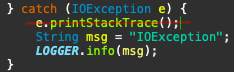
\includegraphics[scale = 0.6]{Logger_info.png}

  \caption {Solução do problema de \textit{Override} do método \textit{hashCode}}

  \label {fig09}

\end{figure}

\end{itemize}

\subsection{CodeSmells}

\subsubsection{Critical CodeSmells:}
\begin{itemize}
\item Possuir um método complexo com cerca de de 290 linhas, é muito difícil manter e até mesmo perceber um código tão extenso.\newline
 Ficheiro: Controller.java\newline

\par Para resolver o problema cada case do \textit{switch} foi dividido em 1 função de complexidade inferior de média 15 linhas. podemos ver nas duas figuras em baixo, um dos cases e a função para o qual foi passado o código correspondente.

\begin{figure}[H]

  \hbox{\hspace{+1em}  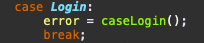
\includegraphics[scale = 0.5]{newSmallerCase.png}}
  \centering
  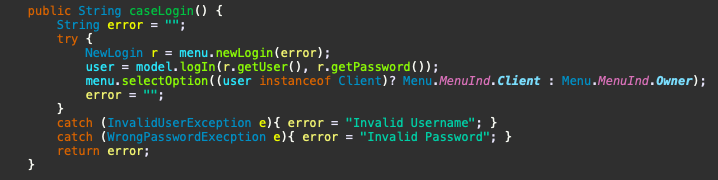
\includegraphics[scale = 0.45]{newSmallerFunction.png}
  \caption {Solução do problema de complexidade extrema do método run()}

  \label {fig10}

\end{figure}
\end{itemize}

\begin{itemize}
\item Repetir várias vezes a atribuição da mesma string pode tornar o código confuso e ineficiente. \newline
\par Para ultrapassar essa dificuldade essa string passou a ser criada e guarda numa constante quando um objeto da classe é inicializado e essa constante é depois atribuída quando necessário. \newline
 Ficheiros: Controller.java, Rental.java, Weather.java e Menu.java\newline
\end{itemize}

\begin{itemize}
\item Usar switch sem caso \textit{default:}. Bastou substituir o ultimo \textit{case "...":} por \textit{default:} para cumprir o mesmo objetivo do código anterior. No caso do ficheiro Menu.java o default foi adicionado após todos os cases existentes para garantir que o programa corria da forma correta.\newline
 Ficheiros: Controller.java, Car.java, Parser.java e Menu.java\newline
\end{itemize}

\begin{itemize}
\item Ter constantes numa enumeração escritas em letras minúsculas. Basta escreve-las em maiúsculas para que passem a seguir a convenção. Para além disso todas as ocorrências destas palavras sofrerão a mesma modificação.
 Ficheiros: Car.java e Menu.java\newline
\end{itemize}

\begin{itemize}
\item Atualizar uma variável static através de um método não estático.\newline
 Ficheiro: Rentals.java\newline
\par Para contornar este problema, transformou-se a variável \textit{static private int id} em \textit{private int id}.
\end{itemize}




\subsubsection{Major CodeSmells:}

\begin{itemize}
\item A existência de blocos try/catch vazios não afeta o desempenho da aplicação mas pode ser um erro de falta de código, neste caso, assumimos que foi deixado propositadamente vazio, logo para não alterar o código restante preencheu-se o bloco com a atribuição de uma String vazia á variável erro.\newline
 Ficheiros: Controller.java e Main.java\newline

 \begin{figure}[H]

  \centering

  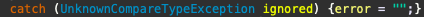
\includegraphics[scale = 0.6]{catchBlockFill.png}

  \caption {Preenchimento do bloco vazio com uma linha de código que não afeta a aplicação}

  \label {fig11}

\end{figure}
\end{itemize}

\begin{itemize}
\item A existência de blocos \textit{try/catch} dentro de um case não é uma boa prática, deve-se criar um método e usar o \textit{try/catch} dentro desta, sendo depois o método chamado dentro do case.\newline
 Ficheiros: Parser.java\newline
\par Para corrigir isto basta criar o método com o bloco \textit{try/catch} lá dentro.
\end{itemize}

\begin{itemize}
\item A utilização de uma classe que reporta uma excepção e não estende a class \textit{Exception} viola a convenção, para corrigir o erro mudou-se a expressão \textit{extends Throwable} para \textit{ extends Exception}.\newline
 Ficheiros: InvalidNewRentalException.java e InvalidNumberOfArgumentsException.java\newline

\par O código corrigido é apresentado na seguinte figura.

 \begin{figure}[H]

  \centering

  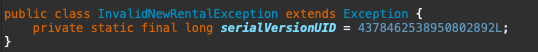
\includegraphics[scale = 0.6]{exceptionCorrection.png}

  \caption {Troca de Throwable por Exception}

  \label {fig12}

\end{figure}
\end{itemize}

\begin{itemize}
\item A utilização de uma classe que reporta uma excepção e não entende a class \textit{Exception} viola a convenção, para corrigir o erro mudou-se a expressão \textit{extends Throwable} para \textit{ extends Exception}.\newline
 Ficheiros: InvalidNewRentalException.java e InvalidNumberOfArgumentsException.java\newline

\par O código corrigido é apresentado na seguinte imagem.

 \begin{figure}[H]

  \centering

  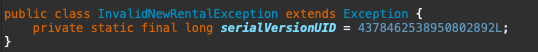
\includegraphics[scale = 0.6]{exceptionCorrection.png}

  \caption {Troca de Throwable por Exception}

  \label {fig13}

\end{figure}
\end{itemize}

\begin{itemize}
\item Ao reportar algo o utilizador deve ser capaz de aceder aos logs facilmente,estes logs têm de ter um formato uniforme, devem ser guardados e dados sensíveis devem ser guardados de forma segura. A utilização de System.out.println() pode comprometer um destes aspetos. Portanto tivemos de importar a biblioteca -textit{java.util.logging.Logger} e criar um \textit{Logger} para guardar o output disponibilizado ao utilizador.\newline
 Ficheiros: Main.java e  Menu.java\newline

\par O código com o Logger é apresentado na seguinte imagem.

 \begin{figure}[H]

  \centering

  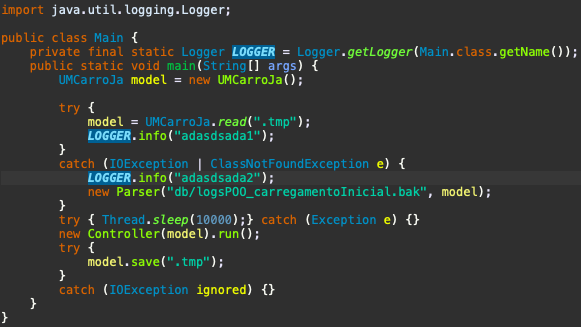
\includegraphics[scale = 0.6]{logger.png}

  \caption {Uso de Logger para seguir requerimentos dos outputs}

  \label {fig14}

\end{figure}
\end{itemize}

\begin{itemize}
\item A utilização de muito parâmetros pode significar que esta classe está a fazer muitas coisas. \newline
Ficheiros: Car.java e RegisterCar.java\newline


\par Achamos por bem para já não alterar este codeSmell, pois a função recebe 9 argumentos quando só devia receber no máximo 7. O excesso de parâmetros não prejudica o desempenho de forma alguma.

\end{itemize}

\begin{itemize}
\item A presença de métodos que não são utilizados (dead code) deve ser removida. \newline
Ficheiros: Point.java e StringBetter.java \newline

\par Na figura em baixo podemos ver um exemplo dos métodos removidos. Na classe StringBetter.java removeu-se o método setStr().
 \begin{figure}[H]

  \centering

  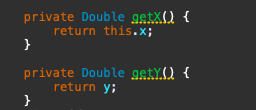
\includegraphics[scale = 0.6]{removedMethods.png}

  \caption {Métodos removidos da classe Point.java}

  \label {fig15}

\end{figure}
\end{itemize}

\begin{itemize}
\item A presença de uma variável com o mesmo nome da classe em que se insere pode confundir, as boas práticas indicam que devem ser nomes distintos. Portanto a variável \textit{menu} foi renomeada para \textit{mymenu}. \newline
Ficheiro: Menu.java \newline

\end{itemize}

\subsubsection{Minor CodeSmells:}
\begin{itemize}
\item Nomes de pacotes com letras maiúsculas.\newline
 Ficheiros: todos os packages excepto o main.java.\newline


\par Para resolver este problema basta substituir as letras maiúsculas nos nomes dos packages por minúsculas, o eclipse trata de renomear o nome do package nas declarações feitas dentro dos ficheiros do próprio package.\newline
\par Em seguida temos um exemplo da correção de uma dessas ocorrências. 
\begin{figure}[H]

  \centering

  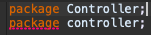
\includegraphics[scale = 0.6]{packageRename.png}

  \caption {Solução do problema de renomear packages}

  \label {fig16}

\end{figure}

\end{itemize}

\begin{itemize}
\item Utilização de métodos ineficientemente.\newline
 Ficheiros: Controller.java e Menu.java.\newline


\par Neste caso num if é utilizado o método size() do ArrayList e seguidamente verifica-se se o array está vazio. A solução para esta ineficiência passa por invocar o método isEmpty() do ArrayList.\newline
\par Em seguida temos um exemplo da correção de uma dessas ocorrências. 
\begin{figure}[H]

  \centering

  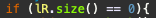
\includegraphics[scale = 0.6]{sizeForIsEmpty.png}

  \caption {Solução do problema de ineficiência no uso de funções de Coleções na classe Controller}

  \label {fig17}

\end{figure}


\par Como na classe \textit{Menu.java} foi preciso trocar a execução do if com o else, para uma melhor percepção do que foi feito, a mudança será mostrada no figura seguinte.

\begin{figure}[H]

  \centering

  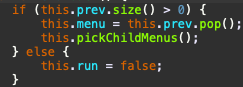
\includegraphics[scale = 0.6]{ifElseChangePre.png}
  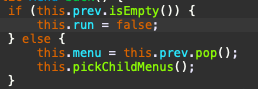
\includegraphics[scale = 0.6]{ifElseChangePos.png}

  \caption {Solução do problema de ineficiência no uso de funções de Coleções na classe Menu}

  \label {fig18}

\end{figure}

\end{itemize}

\begin{itemize}
\item Classe sem package.\newline
 Ficheiro: main.java.\newline


\par Neste caso basta declarar o package a que a classe pertence, como se pode ver na figura seguinte.\newline 

\begin{figure}[H]

  \centering

  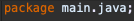
\includegraphics[scale = 0.6]{packageMainJava.png}

  \caption {Declaração do package a que a classe main.java pertence}

  \label {fig19}

\end{figure}

\end{itemize}

\begin{itemize}
\item Utilização de métodos ineficientemente.\newline
 Ficheiro: Car.java.\newline


\par Para colmatar a ineficiência do código basta mudar a negação de uma operação de >, extremamente custosa, para uma operação de >= que tem o mesmo efeito.\newline
\par A resolução encontra-se na figura seguinte. 
\begin{figure}[H]

  \centering

  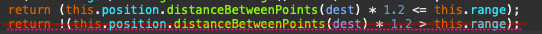
\includegraphics[scale = 0.6]{returnMinorEqual.png}

  \caption {Solução do problema de ineficiência do return}

  \label {fig20}

\end{figure}

\end{itemize}

\begin{itemize}
\item Declaração de um clone() sem implementar Clonable.\newline
 Ficheiros: Car.java, Cars.java, Cliente.java, Owner.java e Point.java.\newline


\par Para resolver o problema basta mudar o nome dest para myclone no método, como se pode ver na seguinte figura.\newline

\begin{figure}[H]

  \centering

  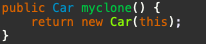
\includegraphics[scale = 0.6]{CloneCar.png}


  \caption {Implementação do método clone() da classe Car}

  \label {fig21}

\end{figure}

\end{itemize}


\begin{itemize}
\item Método devolve ArrayList em vez de List, dando informação sobre a implementação do método.\newline
 Ficheiros: Cars.java e Owner.java.\newline


\par Para resolver o problema basta por o método a devolver uma interface genérica.\newline
\par Note-se que as funções que invocam estes métodos devem ser corrigidas declarando o tipo recebido com \textit{(ArrayList<Rental>)}.

\begin{figure}[H]

  \centering

  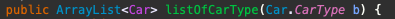
\includegraphics[scale = 0.6]{returningArrayList.png}
  
\includegraphics[scale = 0.6]{returningList.png}

  \caption {Exemplo da mudança do tipo de interface retornada por um método}

  \label {fig22}

\end{figure}

\end{itemize}

\begin{itemize}
\item Utilização desnecessária de parêntesis num filter.\newline
 Ficheiros: Cars.java e UmCarroJa.java.\newline


\begin{figure}[H]

  \centering

  
\includegraphics[scale = 0.6]{filterEpre.png}
  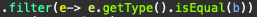
\includegraphics[scale = 0.6]{filterEpos.png}

  \caption {filter sem parêntesis}

  \label {fig23}

\end{figure}

\end{itemize}


\begin{itemize}
\item Declaração de variáveis pela ordem errada, dificultando a leitura do código, estão declaradas da seguinte ordem: static final, final, private. Na figura podemos ver a ordem reescrita da forma correta. \newline
 Ficheiro: Rentals.java.\newline


\begin{figure}[H]

  \centering

  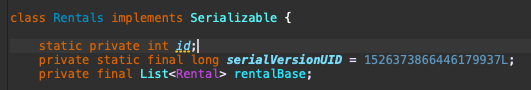
\includegraphics[scale = 0.6]{reorderDeclarations.png}

  \caption {Ordenação correta das declarações de variáveis}

  \label {fig24}

\end{figure}

\end{itemize}

\begin{itemize}
\item Declaração de um método em com a primeira letra maiúscula, o nome Original deste era \textit{RESET()}. \newline
 Ficheiro: StringBetter.java.\newline


\begin{figure}[H]

  \centering

  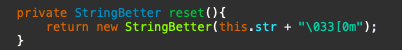
\includegraphics[scale = 0.6]{resetFunction.png}

  \caption {Declaração correta do método, usando letra minúscula no início}

  \label {fig25}

\end{figure}

\end{itemize}

\begin{itemize}
\item Declaração de um método fazendo uso de um underscore no seu nome, seguindo a expressão regular da nomeação de métodos estes não devem ter underscore.De seguida apresenta-se um exemplo de um dos métodos corrigidos. \newline
 Ficheiro: StringBetter.java.\newline


\begin{figure}[H]

  \centering

  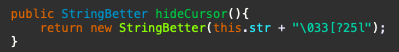
\includegraphics[scale = 0.6]{renameFunction.png}

  \caption {Declaração correta do método retirando o underscore e substituindo letra seguinte por maiúscula}

  \label {fig26}

\end{figure}

\end{itemize}

\begin{itemize}
\item Declaração de variáveis começadas por letra maiúscula. \newline
 Ficheiro: NewLogin.java.\newline

\par Apesar de não ser mostrado, no método NewLogin(), o nome e a password também foram modificado para fazer match com a renomeação demonstrada na figura.

\begin{figure}[H]

  \centering

  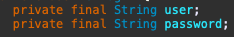
\includegraphics[scale = 0.6]{varsMaiusculas.png}

  \caption {Declaração correta das variáveis user e password}

  \label {fig27}

\end{figure}

\end{itemize}

\subsection{Security Hotspot}

\begin{itemize}

\item A utilização da class \textit{Random} não é segura por permitir que um atacante consiga prever o próximo random gerado e conseguir fazer-se passar por quem não deve.\newline

\par para corrigir este problema bastou substituir a utilização de \textit{Random} por \textit{SecureRandom}.
Ficheiros: Traffic.java e Weather.java

\end{itemize}

\par Adicionalmente foram tratados três problemas referidos pelo IDE Eclipse.

\par O primeiro problema diz respeito ao uso de uma variável error na classe Controller.java. Esta era usada para guardar uma mensagem explicativa do erro ocorrido durante a execução do programa, mas este nunca era mostrado ao utilizador caso ocorre-se. Para isso bastou imprimir caso ocorra, com recurso ao System.out.println(), o erro obtido após um ciclo.\newline

\par No segundo problema existe uma variável "privare int id" no ficheiro Rentals.java que nunca é utilizada para nada, apenas é incrementada quando é adicionado um novo objeto rental mas não tem um propósito no código. Para resolver esta dependência bastou remover esta variável.\newline 

\par Por fim, na classe Menu.java em todos os métodos em que se criava um Scanner este nunca era fechado. Para resolver isto basta fechar o mesmo em todos esses métodos com a adição do código: "scanner.close();" no fim do mesmo.\newline


\subsection{Technical Debts}

Ao fazer a análise dos technical debts foram analisadas versões guardadas no github que tenham sido modificadas de tal forma a que pudesse ter-se dado uma redução do tempo de execução estimado do programa. Os resultados obtidos pelo JStanley são mostrados na figura abaixo.

\begin{figure}[H]

  \centering

  \hbox{\hspace{-8em} 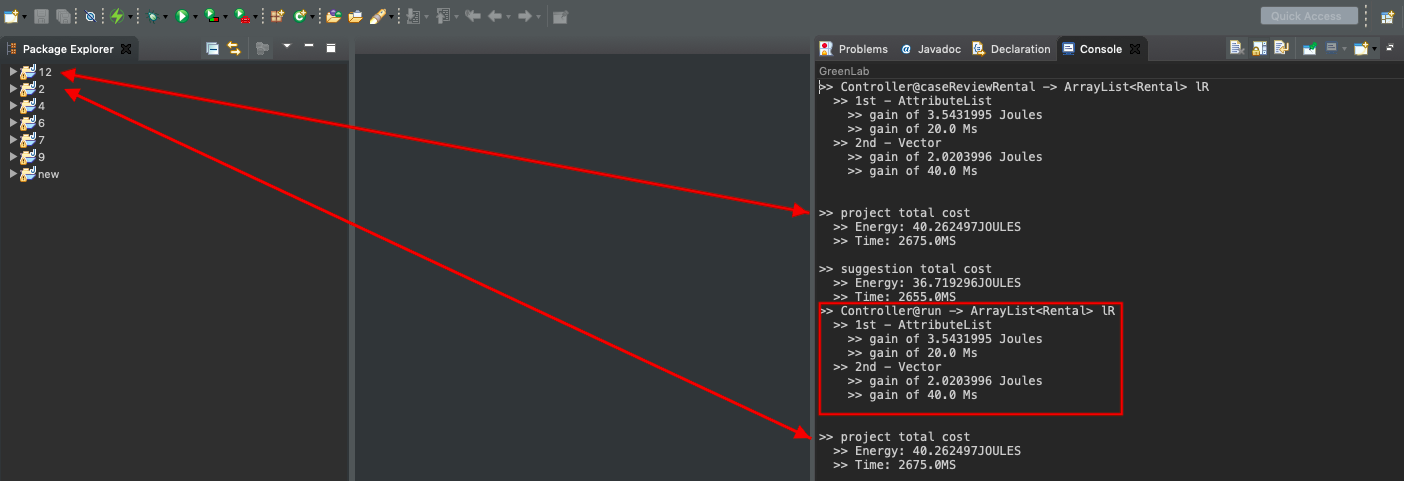
\includegraphics[scale = 0.35]{JStanley'sOutput.png}}

  \caption {Resultados JStanley pré-correção de redSmells}

  \label {fig28}

\end{figure}

\par Como se pode ver pela figura  não se obteve diferença entre as duas versões assinaladas, sendo a 2 a versão com todos os code Smells e bugs originais e a 12 a versão atualmente corrigida (as setas ajudam a visualizar melhor quais os tempos correspondentes). No entanto, convêm atentar que o JStanley detetou formas de melhorar o tempo de resposta da aplicação e/ou de melhorar o custo deste, sendo estas assinaladas por um retângulo. \newline


\par A correção escolhida foi a aplicação de um AtributteList em vez do ArrayList. A leitura após a implementação destas sugestões apresenta-se de seguida assinalada por um retangulo vermelho.\newline

\begin{figure}[H]

  \centering

  \hbox{\hspace{-8em} 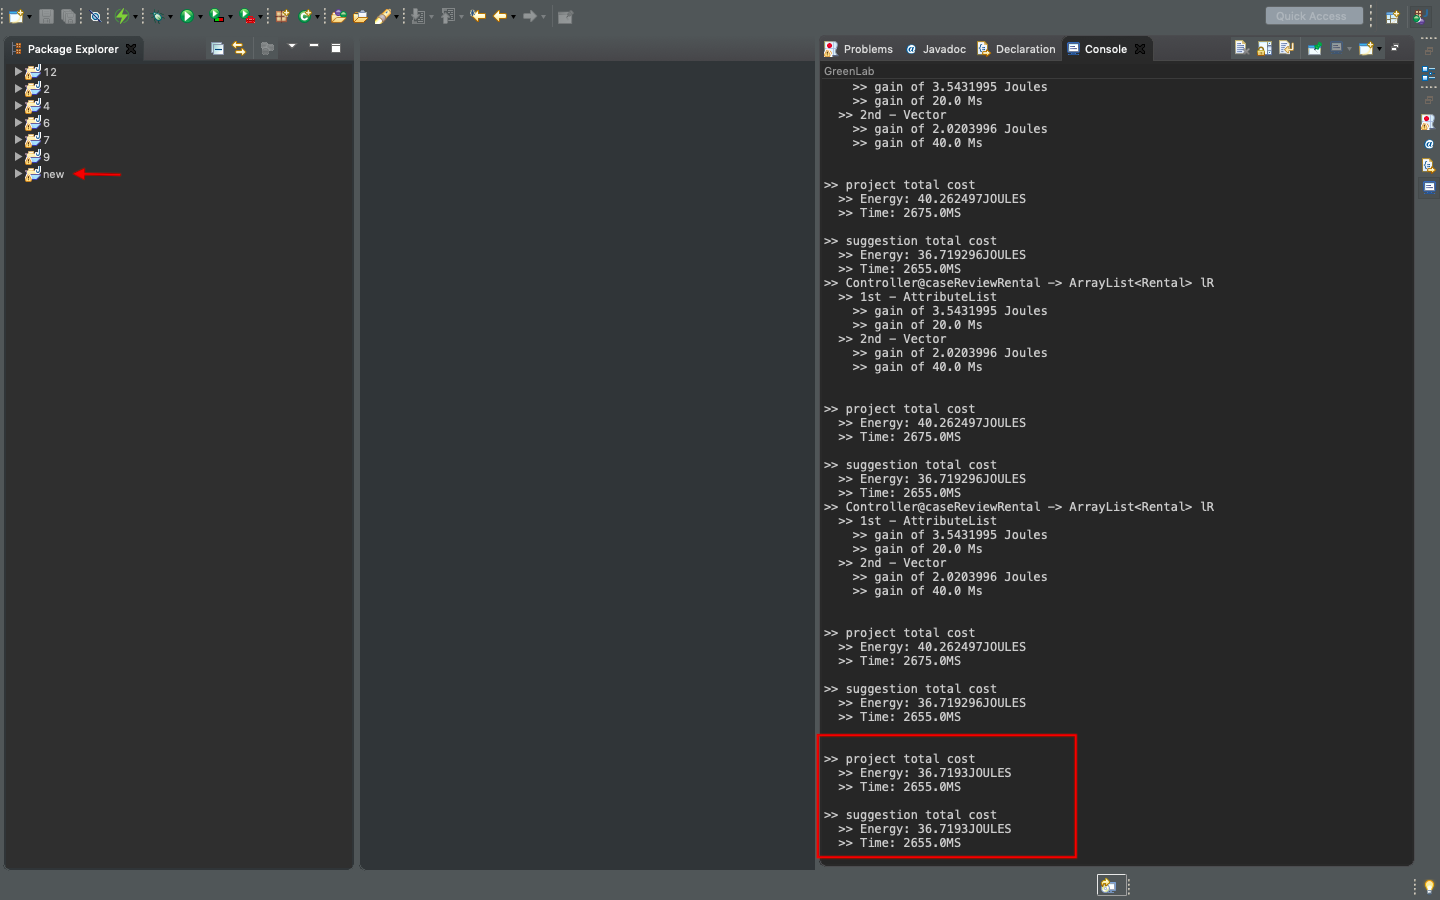
\includegraphics[scale = 0.35]{JStanley'sOutput2.png}}

  \caption {Resultados JStanley pós-correção de redSmells}

  \label {fig29}

\end{figure}

\par Par após todos estes processos de correção de codeSmells e bugs, obtivemos o seguinte resultado no sonarQube.

\begin{figure}[H]

  \centering

  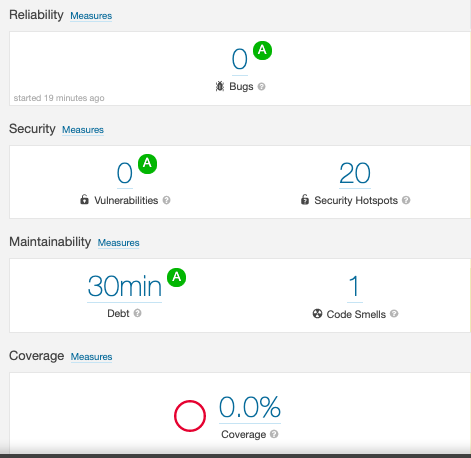
\includegraphics[scale = 0.6]{allFixed.png}

  \caption {Todo o código foi corrigido com sucesso}

  \label {fig27}

\end{figure}
\newpage